\documentclass[a4paper,11pt]{article}
\usepackage{fancyhdr}
\usepackage[utf8]{inputenc}
\usepackage{color}
\usepackage{pgf}
\usepackage{tikz}
\usepackage{graphicx}
\usepackage{multirow}
\usepackage{listings}
\usetikzlibrary{arrows, automata}
\lstset{keywordstyle=\color{blue},language=VHDL}
\setlength{\headheight}{5pt}

\lhead
\rhead
%\parskip 1em
%\parindent 0em

\begin{document}
%\pagestyle{empty}
%-----------------------------------------------------------
\begin{titlepage}

\title{\Huge{Lab report} \\[0.1cm] \Large{Digital Design (EDA322)}}
\author{\large{\emph{Group 01}} \\[0.2cm] Erik Thorsell1 \\[0.05cm] Robert Gustafsson \\[0.1cm]}
\maketitle
\thispagestyle{empty}
\end{titlepage}
\clearpage
%-----------------------------------------------------------
\pagestyle{fancyplain}
\pagenumbering{roman}
\tableofcontents
\clearpage
\pagenumbering{arabic}
\setcounter{page}{1}

\section{Introduction}
Understanding the complex architecure of a modern central processing unit can 
seem difficult, at best. This report aims to give a brief introduction to 
the functionality, development process and finished version of the ChAcc 
processor. The report covers the development of: the ALU and its parts, 
the design of the registers and memory components, the bus and the controller 
unit. The finished product was later tested exstensively and programmed onto an 
FPGA (Field-Programmable Gate Array). The last two sections covers this.

\section{Method}
\subsection{Arithmetic and Logic Unit (ALU)}
The ALU (Arithmetic and Logic Unit) is one of the core components in a CPU 
(Central Processing Unit). As the name vouches the ALU is in control of the 
operations between operands. An ordinary ALU does arithmetic as well as logic 
operations, however the ChAcc (Chalmers Accumulator) processor comes with a 
slightly reduced set of instructions. Because of this the ChAcc ALU is limited 
to the operations: addition, subtraction as well as the logical operations nand 
(not and), not, aswell as a comparison operation. One should also note that 
the operations are only supported for unsigned numbers.\\\\
\noindent
The purpose of the laboration was to implement the ALU, mentioned above, in 
VHDL. Broken into several stages the first one was to implement an RCA (Ripple 
Carry Adder), composed of multiple full adders. Briefly, an RCA is a simple 
adder that can easily be scaled to handle input of various sizes. This is since 
an RCA is simply a chain of full adders that each takes three bits as input 
and returns the sum of them aswell as a carry out. These inputs are the two 
bits that are to be added aswell as a carry in. In our case the inputs to the 
ALU are composed of two eight bit, unsigned, numbers leaving us with total 
of eight full adders in the chain.

\begin{figure}[h]
    \centering
    
\includegraphics[scale=0.25]{FA.png}
    \caption{A full adder, decscribed with logical gates.}
    \label{FA}
\end{figure}

\noindent
Using the dataflow design for our full adders the logic was pretty straight 
forward. The truth table, given in the laboration description, for a full 
adder speaks for itself and after minimizing the table we moved onto the more 
interesting part of the laboration, the RCA.\\\\
\noindent
The structural design style of VHDL lets one create instances of already 
programmed components and was used to create the RCA. After creating eight 
instances of the full adder it was simply a matter of passing the right 
arguments to each of the full adders. The least significant bit of each input 
gets send to the first full adder, along with the carry in, which returns the 
least significant bit of the sum as well as a first carry out. The second to 
least significant bits of each input is then send to the second full adder 
along with the carry out from the first full adder. This is repeated eight 
times and the carry out of the eigth full adder is the carry out of the RCA. 
The correctness of the RCA was easily verified by the use of a ''do-file''.

\begin{figure}[h]
    \centering
    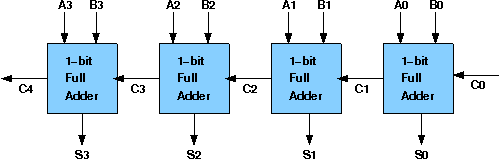
\includegraphics[width=\linewidth]{RCA.png}
    \caption{A ripple carry adder, composed out of 4 full adders.}
    \label{RCA}
\end{figure}

\noindent
The comparison operation compares two operands and calculates wether or not 
they are equal. When this is done the corresponding flag (Equal, EQ or Not 
Equal, NEQ) is asserted. Implementing the component was straight forward and 
since the instructions specifies one must not use the behavioral design style 
we opted to use the dataflow style. A {\it for .. generate} statement was used 
to improve readability aswell as reduce the amount of code in the file. A 
bitwise comparison checks if the {\it n:th} bit of any input differs by the 
use of an xor gate. For every iteration of the loop, the output of the gate is 
stored in a temporary signal which is then also used in the loop by the use 
of an or operation which is done with the new result and the old.\\\\
\noindent
When the loop is done the temporary signal is asserted to the EQ flag, and it 
is a simpe matter of inverting the signal to get the NEQ flag.\\\\
\noindent
The third task of the laboration was composed of writing the implementation 
for the subtraction, the not and nand operations, as well as an {\it isOutZero} 
signal. Ofcourse one also has to be able to choose between the 
operations, this ability  was implemented using a 4-to-1 multiplexer.\\\\
\noindent
The subtraction operation was simply a matter of performing an addition with 
one of the operands {\it two complements representation}. This is achieved by 
inverting the operand and then add 1 to it. An xor with eight ones with one of 
the operands as well as adding a carry in to the RCA input solves this. The 
nand operation is self explained and is achieved by inverting an and with the 
two operands. The not operation returns the first operand ({\it ALU\_inA}) 
inverted. {\it isOutZero} is done by performing a bitwise or of the output 
from the multiplexer.

\subsection{Top-level Design}
Implementing the top-level design of the ChAcc processor included the 
implementation of storage components, such as memory, registers and the 
bus, as well as initializing the memory components, and connecting all the 
datapath components together.\\\\
\noindent
Firstly we created a generic register with asynchronus reset making use 
of the behavioral design in VHDL. A simple process, triggered by either 
the clock or the reset signal, firstly checks if the register is to be reseted 
or not. The register will be reset if and only if the reset signal is 0. 
However if the reset signal is 1 the process checks if the clock signal was 
caused by a rising edge and if that is the case the register will be written 
to if, and only if, the registers load signal is 1.

\begin{lstlisting}[frame=single]
PROCESS(ARESETN, CLK)
    BEGIN
        IF ARESETN = '0' THEN
            output <= (OTHERS => '0');
        ELSIF rising_edge(CLK) THEN
            IF loadEnable = '1' THEN
                output <= input;
            END IF;
        END IF;
END PROCESS;
\end{lstlisting}

\noindent
A register holds only one signal at the time so for larger portions of data 
the ChAcc has two memories - one for the instructions and one for the data. 
ChAcc has two memories instead of one since it follows the Hardvard 
architecture. however making use of generics - as with the register - we only 
had to implement one, and when implementing the top-level design we 
instanciated the two memories with generic maps and different init files.\\\\
\noindent
The processor bus was implemented using a 4 to 1 multiplexer along with some 
extra logic to incorperate the four control signals into one bit. We mimized 
the expression with the four signals and opted to default to the EXTDATA 
signal. Two or gates were needed to get the desired functionality.

\subsection{Controller}
While designing the top level of the ChAcc processor we were provided with a 
{\it mock controller}, that acted purely as a place holder. However when that 
asignment was done we were to implement our very own controller. The 
controller is used to pass the correct instructions to the correct components 
of the ChAcc processor at the right time. In order to accomplish this we 
implemented a Mealy machine, divided into three processes. A Mealy machine is 
an FSM (Finite-State Machine) whose output values depends both on the current 
state - as well as the current input - of the machine. A complete diagram of 
the FSM, as well as code examples for the three processes, can be found in 
the appendix.\\\\
\noindent
The ChAcc processor's specification documentet provided describes the working 
of the controller, and the document also specifies which signals are to be set 
and reset during which operations. This information is crucial in order to 
implement the controller and was of great use to us.\\\\
\noindent
When the controller was implemented we were provided with a testbench to be 
run in the simulation software. The testbench tested a couple of operations 
e.g. adding, subtracting, reading and writing from memory, etc. Unfortunately 
our processor did not pass the test on our first attempt and we spend many 
hours trying to figure out why. The problem was finally solved by rewriting 
our FSM. Our first implementation made use of some logical minimization in 
order decide what state to enter, however the software seemed not to approve 
of this and our final implementation uses a simple case statement instead.

\subsection{Processor's Testbench}
In order to test the correctness of our implementation of the ChAcc processor 
we created a testbench. We were with provided two files to initialize our 
memories with, as well as five files to compare the output of our ChAcc 
processor with.\\\\
\noindent
The testbench is divided into three parts. A reading part, a comparison part 
and a round up part. For each ''comparision file'' we created one reading 
process and one comparison process. The reading process simply reads each 
line of the provided file and transforms the given row into a standard 
logic vector which can be compared to the output of the ChAcc processor. 
When the reading process is done a boolean that was initialized to false 
is set to true, this is to show that we have reached the end of the file.

\begin{lstlisting}[frame=single]
readAcc: PROCESS
    VARIABLE accLine : LINE;
    VARIABLE accData : BIT_VECTOR(7 DOWNTO 0);
BEGIN
    FOR i IN 1 TO 30 LOOP
        WAIT UNTIL (ARESETN = '1' AND rising_edge(CLK);
            READLINE(accFile, AccLine);
            READ(accLine, accData);
            WAIT UNTIL (acc2seg'ACTIVE);
               accSignal <= TO_STDLOGICVECTOR(accData);
    END LOOP;
    accEOF <= true;
    WAIT;
END PROCESS;
\end{lstlisting}

\noindent
The comparison process checks if we have reached the end of the file 
corresponding to the process. If that is not the case we compare the 
output from the read file with the signal from the ChAcc processor. 
If they differ an error has occured and we report this to the user, 
the testbench also terminates due to the severity of the error.\\\\
If no errors occur throughout the comparison process we simply move 
on and we wait for the other processes to finish.

\begin{lstlisting}[frame=single]
verifyAcc : PROCESS(CLK)
BEGIN
    IF (not accEOF and ARESETN = '1' 
        and falling_edge(CLK)) THEN
        IF (acc2seg /= accSignal) THEN
                accBool <= accBool and false;
                REPORT "Acc ERROR"
                SEVERITY ERROR;
        ELSE
            accBool <= accBool and true;
        END IF;
    END IF;
END PROCESS
\end{lstlisting}

\noindent
When all the comparisons are done the test is complete. The 
end process makes sure that all the comparisons were true and 
prints a note that tells the user that the test succeeded. When 
this is done the testbench terminates with the message ''TEST DONE''.\\\\
\noindent
Since every iteration of the comparison process also checks the 
validness of the signal there is really no need to check the validness 
of all the booleans but you should always cover your bases.

\begin{lstlisting}[frame=single]
endProcess : PROCESS(CLK)
    IF accEOF and dispEOF and dmemEOF and 
       flagEOF and pcEOF THEN
        IF NOT accBool OR
           NOT dispBool OR
           NOT dmemBool OR
           NOT flagBool OR
           NOT pcBool THEN
               REPORT "NOT CORRECT"
               SEVERITY NOTE;
           ELSE
               REPORT "TEST SUCCEEDED"
               SEVERITY NOTE;
        END IF;
        REPORT "TEST DONE"
        SEVERITY FAILURE;
    END IF;
END PROCESS
\end{lstlisting}

\subsection{ChAcc on Nexys 3 board \emph{(Optional)}}
(max: 2 pages)
\\\\
Describe how you verified the correctness of your FPGA implementation. Note that the code that is executed on the implementation is the same code used for testing in Lab 5. You should compare sequences of values on various signals observed on the seven-segment displays to values seen in Modelsim simulation of the design. Please include in the report the sequence of program counter (PC) and display register values you observed during a successful execution on the FPGA. 

\subsection{Performance, Area and Power Analysis \emph{(Optional)}}
(max: 2 pages)
\\\\
To be announced in the Lab7PM.

\section{Analysis}
(max: 1 page)
\\\\
Summarize your results after performing all the labs (2, 3, 4 and 5).

Mention and discuss interesting findings and observations, as well as difficulties in completing some of the tasks of the four last labs.

After looking at your results, draw conclusions and describe briefly the learning outcome, that is what have you learnt by performing these labs?  

% Appendix
\newpage
\begin{appendix}

\section{Appendix}

\begin{figure}[h]
\centering
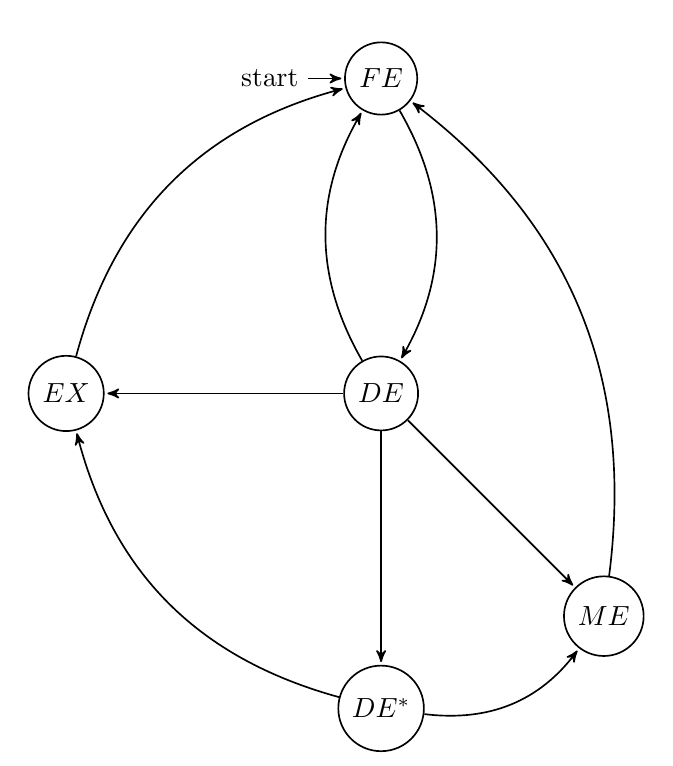
\begin{tikzpicture}[->, >=stealth', shorten >=1pt, auto, node distance = 4cm, semithick]
    \node[initial, state]   (FE)            {$FE$};
    \node[state]   (DE)   [below of=FE]     {$DE$};
    \node[state]   (DES)  [below of=DE]      {$DE^*$};
    \node[state]   (EX)   [left of=DE]     {$EX$};
    \node[state]   (ME)   [below right of=DE]     {$ME$};

    \path (FE) edge [bend left] node {} (DE)
          (DE) edge [] node {} (DES)
          (DE) edge [bend left] node {} (FE)
          (DE) edge [] node {} (EX)
          (DE) edge [] node {} (ME)
          (DES) edge [bend left] node {} (EX)
          (DES) edge [bend right] node {} (ME)
          (EX) edge [bend left] node {} (FE)
          (ME) edge [bend right] node {} (FE);
\end{tikzpicture}
\caption{Mealy Finite-State Machine.}
\end{figure}
\vspace{1cm}
\begin{lstlisting}[frame=single]
PROCESS(CLK, ARESETN)
BEGIN
IF ARESETN = '0' THEN
    current_state <= FE;
ELSE
    IF (rising_edge(CLK) THEN
        IF master_load_enable = '1' THEN
            current_state <= next_state;
        END IF;
    END IF;
END IF;
END PROCESS    
\end{lstlisting}
\vspace{1pt}
\center {\it The first third of the FSM.}

\newpage

\begin{tabular}{|l|l|l|}
\hline
\multicolumn{3}{ |c| }{Mealy FSM} \\
\hline
State & Opcode & Signals \\ \hline
\hline
\multirow{7}{*}{FE} 
& 000X, 0101, 0110, 100X, 1111 & instrLd \\
& 0010 & instrLd, aluMd(0) \\
& 0011 & instrLd, aluMd(1) \\
& 0100 & instrLd, aluMd(1), aluMd(0) \\
& 0111, 1010 & instrLd, acc2bus \\
& 1011 & instrLd, ext2bus \\
& 1100 - 1110 & instrLd, im2bus \\
\hline
\multirow{9}{*}{DE} 
& 000X, 0101, 0110, 1001 & instrLd, dataLd \\
& 0010 & instrLd, dataLd, aluMd(0) \\
& 0011 & instrLd, dataLd, aluMd(1) \\
& 0100 & instrLd, dataLd, aluMd(1), \\
&      & aluMd(0) \\
& 0111 & instrLd, acc2bus \\
& 1010 & instrLd, dataLd, acc2bus \\
& 1011 & pcLd, instrLd, dmWr, ext2bus \\
& 110X, 1110 & pcSel$^*$, pcLd, instrLd, im2bus \\
& 1111 & instrLd \\
\hline
\multirow{2}{*}{DE*} 
& 100X & instrLd, addrMd, dataLd\\
& 1010 & instrLd, acc2bus \\
\hline
\multirow{9}{*}{EX} 
& 000X & pcLd, instrLd, flagLd, accLd, \\
&      & dmRd \\
& 0010 & pcLd, instrLd, flagLd, accLd, \\
&      & dmRd, aluMd(0) \\
& 0011 & pcLd, instrLd, flagLd, accLd, \\
&      & dmRd, aluMd(1) \\
& 0100 & pcLd, instrLd, flagLd, accLd, \\ 
&      & aluMd(1), aluMd(0) \\
& 0101 & pcLd, instrLd, flagLd, dmRd \\
& 0110 & pcLd, instrLd, accSel, accLd, \\
&      & dmRd \\
& 1000 & pcLd, flagLd, accLd, dmRd \\
& 1001 & pcLd, flagLd, accSel, accLd, \\
&      & dmRd \\
& 1111 & pcLd, instrLd, dispLd \\
\hline
\multirow{2}{*}{ME}
& 0111 & pcLd, instrLd, dmWr, acc2bus \\
& 1010 & pcLd, instrLd, addrMd, \\
&      & dmWr, acc2bus \\
\hline
\end{tabular}
\center {\it The complete table of states and corresponding signals.}

\newpage

\begin{lstlisting}[frame=single]
PROCESS(current_state, opcode)
BEGIN
CASE current_state IS
    WHEN FE =>
        next_state <= DE;
    WHEN DE =>
        CASE opcode IS
            WHEN "0000" => next_state <= EX;
            WHEN "...." => next_state <= ..;
        END CASE;
    WHEN DES =>
        CASE opcode IS
            ...
        END CASE;
    WHEN ...
END CASE;
END PROCESS    
\end{lstlisting}
\center {\it The second part of the FSM.}
\vspace{30pt}
\begin{lstlisting}[frame=single]
PROCESS(current_state, opcode)
BEGIN
CASE opcode IS
    WHEN "0000" =>
        CASE current_state IS
            WHEN FE =>
              v_control <= (2 => '1', others => '0');
            WHEN DE =>
              v_control <= (2 | 5 => '1', 
                            others => '0');
            WHEN EX =>
              v_control <= (1 | 2 | 6 | 8 | 10 => '1', 
                            others => '0');
        END CASE;
    WHEN .... =>
END CASE;
END PROCESS    
\end{lstlisting}
\center {\it The third part of the FSM.}
\vspace{25pt}

\newpage

\end{appendix}

\end{document}
